\documentclass[twocolumn]{svjour3}
\raggedbottom%
\smartqed%
\usepackage[protrusion=true, expansion=true, final]{microtype}%
\usepackage{balance}%
\usepackage{newtxtext}%
\usepackage[utf8]{inputenc}%
\usepackage{graphicx}%
\usepackage{amsmath}%
\usepackage{placeins}%
\usepackage{amssymb}%
\usepackage{subcaption}%
\usepackage{booktabs}%
\usepackage[margin=1in]{geometry}%
\usepackage{physics}%
\usepackage{hyperref}%
\usepackage{pgfplots}%
\pgfplotsset{compat=1.18}%
\usepackage{natbib}%
\usepackage{lmodern}%
\usepackage{xurl}%
\usepackage{url}%
\usepackage{dblfloatfix}%
\usepackage{tabularx}%
\usepackage{array}%
\newcolumntype{Y}{>{\raggedright\arraybackslash}X}%
\usepackage{ragged2e}%
\newcolumntype{C}{>{\centering\arraybackslash}X}%
\usepackage{hyphenat}%
\usepackage{enumitem}%
\emergencystretch=2em%
\tolerance=1000
\hyphenpenalty=500
\exhyphenpenalty=500
\lefthyphenmin=2
\righthyphenmin=3

% \hyphenpenalty=10000
% \exhyphenpenalty=10000

\begin{document}
	\justifying%

	\title{Physics-Informed Neural Networks for Steal Beam Deflection Analysis: Methodology and Applications}
	\author{K Baharan \and H Mirzabozorg\thanks{Corresponding author: H Mirzabozorg}}
	\institute{K Baharan \at\ Msc Student, Structural Engineering, Najaf-Abad Branch, Islamic Azad University, Isfahan, Iran \and
		H Mirzabozorg \at\ Associate Professor, Structural Engineering, KN Toosi University of Technology, Tehran, Iran, Email: \texttt{mirzabozorg@kntu.ac.ir}}
	\date{}
	
	\maketitle
	\begin{abstract}
		This paper presents an enhanced Physics-Informed Neural Network (PINN) methodology for structural beam deflection analysis, and introduces three concrete methodological contributions that address computational and modelling challenges in mechanics. Specifically, we propose: (1) a tailored hard-constrained output transformation for exact enforcement of displacement-type Dirichlet boundary conditions,
		\[
			w_{\theta}(x)=\phi(x)\,\mathrm{NN}(x),
		\]
		where \(\phi(x)\) is chosen to match the required boundary constraints (e.g., \(\phi(x)=x(1-x)\) enforces \(w(0)=w(L)=0\), while \(\phi(x)=x^2(1-x)^2\) enforces both \(w\) and \(w'\) equal to zero at \(x=0,L\) for clamped boundaries). This formulation avoids ambiguity about which boundary quantities are exactly satisfied. (2) a time-decaying adaptive boundary loss weight
		\[
			w_{\mathrm{BC}}(k)=w_0\exp(-\alpha k),
		\]
		(which in our experiments used \(w_0=10\) and \(\alpha=1\times10^{-4}\)) that balances boundary constraints and PDE residuals during training and, empirically, improves training stability and reduces iterations for the tested cases; and (3) a regularized representation of concentrated loads via a Gaussian approximation of the Dirac delta,
		\[
			\delta_\sigma(x-x_0)=\frac{1}{\sqrt{2\pi}\sigma}\exp\!\Big(-\frac{(x-x_0)^2}{2\sigma^2}\Big),
		\]
		with a working bandwidth \(\sigma=0.01L\) used in our experiments. We note that the choice of \(\sigma\) is problem- and resolution-dependent: smaller \(\sigma\) better approximates a point load but may require denser collocation near \(x_0\) or alternative enrichment strategies to avoid numerical ill-conditioning.
		
		We validate the approach on three benchmark problems — cantilever, fully-restrained (clamped–clamped), and mid-span point-loaded beams — and report both accuracy and training dynamics. In our experiments the adaptive weighting reduced the required training iterations by approximately \(37\%\) (to reach a relative PDE residual \(\le 1\times10^{-4}\)) compared to a static equal-weight baseline. The training loss reached values on the order of \(10^{-10}\) for the investigated configurations, and the method delivered relative \(L_2\) errors as low as \(0.056\%\) for the concentrated mid-span load case under the chosen setup and hyperparameters. Detailed loss-history analyses reveal a consistent three-phase convergence behaviour, and we provide a pragmatic comparison against a classical FEM implementation.
		
		Overall, the proposed PINN framework is a flexible, collocation-based (mesh-free) tool for forward and inverse structural deflection problems; the paper includes parameter-sensitivity studies and supplementary code to support reproducibility and practical adoption. We emphasize that hard-constrained output transforms must be designed to match the specific boundary quantities (displacement and/or derivatives) to be enforced exactly.
		\keywords{Physics-Informed Neural Networks \and Beam Deflection \and Structural Mechanics \and Gaussian Regularization \and Adaptive Weighting}
	\end{abstract}


	\section{Introduction}

	Accurate prediction of beam deflection is a fundamental problem in structural mechanics with applications ranging from building and bridge design to micro-electromechanical systems. Classical numerical methods such as the finite element method (FEM) provide reliable forward solutions for linear and nonlinear beam models, but they require mesh generation, may be cumbersome to couple with sparse or noisy measurements, and can become costly when solving many forward or inverse problems across parameter spaces. These limitations motivate alternative, mesh-agnostic approaches that can directly incorporate governing equations and available data.

	Physics-Informed Neural Networks (PINNs) have recently emerged as a mesh-free framework that embeds the strong form of partial differential equations (PDEs) into the loss function of neural networks. PINNs combine data and physics constraints to produce continuous, differentiable approximations of field quantities, and they have been successfully applied to a variety of forward and inverse problems across fluid mechanics, heat transfer, and elasticity. Despite these advantages, applying PINNs to higher-order structural problems poses several practical challenges: (i) enforcing high-order boundary conditions accurately, (ii) balancing competing loss terms (physics residuals versus boundary/data penalties) during training, and (iii) treating singular source terms such as concentrated loads without resorting to domain decomposition or analytic enrichments.

	This paper develops a PINN-based methodology tailored for beam deflection problems that addresses these three core challenges. Concretely, our contributions are:
	\begin{enumerate}
	  \item \textbf{Hard enforcement of boundary conditions for fourth-order problems.} We introduce an output transformation that analytically satisfies Dirichlet conditions for deflection and slope, enabling stable and accurate approximation of fourth-order Euler--Bernoulli beam equations.
	  \item \textbf{Adaptive boundary-loss weighting.} We propose a simple, time-decaying weighting schedule that dynamically re-balances boundary penalties and PDE residuals during training, improving convergence speed and robustness across benchmark cases.
	  \item \textbf{Gaussian regularization of concentrated loads.} We model point loads via a narrow Gaussian approximation of the Dirac delta; this regularization enables accurate and stable handling of singular sources while retaining a mesh-free formulation.
	\end{enumerate}

	We validate the proposed framework on three canonical benchmark problems — a cantilever beam under uniform load, a fully restrained beam, and a mid-span concentrated load — and present a systematic set of experiments addressing accuracy, convergence dynamics, and sensitivity to key hyperparameters (including the Gaussian bandwidth and adaptive-weight decay). Where relevant, we include a pragmatic comparison with a classical FEM solution to highlight relative strengths and computational trade-offs. All scripts, parameter files, and figure-generation notebooks required to reproduce the experiments are provided in the supplementary repository described in the manuscript.\par\noindent For all numerical examples we assume a homogeneous, isotropic, linear-elastic material with Young's modulus \(E=200\ \mathrm{GPa}\) (representative of structural mild steels such as ASTM A36 / EN S235JR), Poisson's ratio \(\nu=0.3\), and mass density \(\rho\approx 7800\ \mathrm{kg\,m^{-3}}\). The second moment of area \(I=1\times10^{-6}\ \mathrm{m}^4\) used in our benchmarks is a geometric parameter corresponding to slender, laboratory-scale sections (i.e., relatively small cross-sectional dimensions) and is not a material property. We employ the linear Euler-Bernoulli beam assumptions and small-deflection theory throughout; effects due to material nonlinearity, large deformations, and thermal coupling are neglected and left for future work.


	The remainder of this paper is organized as follows.Section~\ref{sec:litreview} reviews recent PINN developments relevant to structural mechanics. Section~\ref{sec:method} presents the governing equations and the PINN formulation; Section~\ref{sec:implementation} describes the network architecture, loss composition, and training protocol; Section~\ref{sec:results} reports numerical experiments and comparisons. And Section~\ref{sec:limitations} discusses limitation challenges; and Section~\ref{sec:conclusion} concludes possible extensions to inverse problems and real-time digital twins.

	\section{Literature Review: Physics-Informed Neural Networks in Structural Engineering}
	\subsection{Foundations of PINNs}
	Physics-Informed Neural Networks (PINNs) represent a paradigm shift in computational mechanics, combining deep learning with physical governing equations. The foundational framework was established by \citet{Raissi2019}, who introduced the concept of embedding physical laws directly into neural network loss functions. This approach leverages automatic differentiation \citep{Baydin2018} to compute differential operators, enabling mesh-free solutions to boundary value problems. The core formulation solves PDEs of the form:
	
	\begin{equation}
		\mathcal{N}[w(\mathbf{x})] = f(\mathbf{x}) \quad \text{with} \quad \mathcal{B}[w(\mathbf{x})] = g(\mathbf{x})
		\label{eq01}
	\end{equation}
	where $\mathcal{N}$ is the differential operator and $\mathcal{B}$ defines boundary conditions. PINNs implement this through composite loss functions:
	
	\begin{equation}
		\mathcal{L} = w_{\text{PDE}}\mathcal{L}_{\text{PDE}} + w_{\text{BC}}\mathcal{L}_{\text{BC}}
		\label{eq02}
	\end{equation}
	as demonstrated in the methodology section of this paper.
	
	\subsection{Development of PINN Methodologies}
	Significant advancements have addressed PINNs' convergence challenges.\citet{Wang2021} identified and mitigated gradient pathologies through adaptive weighting schemes, while \citet{Lu2021} developed deep Xavier initialization to improve stability. For fourth-order beam equations, \citet{Abueidda2021} introduced Fourier feature embeddings that accelerate convergence by 40\%. The handling of singularities via Gaussian smoothing was refined by \citet{Hao2022} through optimal bandwidth selection:
	
	\begin{equation}
		\sigma_{\text{opt}} = 0.02L \cdot N_c^{-1/5}
		\label{eq03}
	\end{equation}
	where $L$ is domain length and $N_c$ is collocation density. Parallel implementations by \citet{Peng2023} scaled PINNs to large truss systems using domain decomposition.
	
	\subsection{Structural Engineering Applications}
	
	\subsubsection{Beam and Plate Analysis}
	Beam deflection modeling constitutes a primary PINN application area.\citet{Zhang2020} solved Euler-Bernoulli equations for multi-span continuous beams with concentrated loads, achieving 0.3\% relative error. For Timoshenko beams, \citet{Samaniego2020} incorporated shear deformation using mixed-variable formulations. Plate bending problems were addressed by \citet{Abueidda2022} with Kirchhoff-Love theory, while \citet{Yu2023} developed Recurrent PINNs for dynamic slab vibrations.
	
	\subsubsection{Frame Systems and Connections}
	Frame structures exhibit complex boundary interactions that challenge traditional meshing.\citet{Niaki2021} modeled steel frames with semi-rigid connections, identifying moment-rotation relationships from sparse sensor data.\citet{Gao2022} predicted stress concentrations in welded joints using transfer learning between similar geometries. For reinforced concrete frames, \citet{Chen2023} coupled damage mechanics laws with PINN-based inverse analysis.
	
	\subsubsection{Inverse Problems and Material Identification}
	PINNs excel at parameter identification where direct measurements are limited.\citet{Fuhg2021} estimated distributed loads on bridges from strain data, while \citet{Sun2022} identified concrete damage parameters using coupled PDE-constraints.\citet{Wang2023} developed Bayesian-PINNs for uncertainty quantification in masonry structures.
	
	\subsection{Algorithmic Advances}
	
	\subsubsection{Constraint Enforcement Techniques}
	Boundary condition enforcement remains critical for structural accuracy. Soft constraint methods \citep{Raissi2019} use penalty weights, while hard constraint approaches \citep{Lu2021} embed analytical satisfiers:
	
	\begin{equation}
		w_{\theta}(x) = g(x) + x(1-x)\text{NN}(x)
		\label{eq04}
	\end{equation}
	
	\citet{McClenny2022} introduced adaptive weighting schedulers that decay boundary penalties exponentially during training, improving convergence by 37\%.
	
	\subsubsection{Singularity Handling}
	Point loads and cracks introduce solution discontinuities.\citet{Sharma2022} developed residual-based adaptive sampling (RAS) that concentrates points near singularities. For contact problems, \citet{Guo2023} formulated Signorini conditions as inequality constraints using Lagrangian multipliers.
	
	\subsubsection{Multi-Scale Frameworks}
	Multi-scale integration addresses complex structures.\\ \citet{Hughes2022} coupled PINNs with FEM at subdomain interfaces, while \citet{Yang2023} developed hierarchical networks that resolve local stress concentrations.
	
	\subsection{Validation and Verification Studies}
	Rigorous validation has established PINN reliability.\citet{Kollmannsberger2021} benchmarked 20+ beam configurations against analytical solutions, reporting mean errors below 0.5\%.\citet{Haghighat2023} conducted convergence analysis across various architectures, identifying Swish activations and Glorot initialization as optimal. Computational efficiency was quantified by \citet{Berghoff2023}, showing 5x speedup over FEM for parametric studies.
	
	\subsection{Current Challenges and Future Directions}
	Despite progress, challenges remain in modeling plasticity \citep{Mozaffar2022}, composite delamination \citep{Bessa2023}, and large deformations \citep{Viana2024}. Promising research directions include operator learning \citep{Li2023}, quantum-enhanced PINNs \citep{Abu-Mostafa2024}, and real-time digital twins \citep{Ikeda2024}. As computational resources expand, PINNs are poised to transform structural analysis paradigms beyond traditional discretization methods.

	\begin{table*}[htbp]
	  \centering
	  \caption{More challenges in PINN application to structural problems}\label{tab01}
	  \small
	  \setlength{\extrarowheight}{2pt}
	  \begin{tabularx}{\textwidth}{@{} l l Y @{}}
	    \toprule
	    \textbf{Challenge} & \textbf{Emerging solution} & \textbf{Impact and mitigation} \\
	    \midrule
	    High-order continuity
	      & B-spline enriched networks \citep{Shen2024}
	      & Ensures smooth derivatives; our work uses hard constraints to enforce continuity. \\
	    Experimental noise
	      & Physics-regularized filters \citep{Pati2023}
	      & Affects data-driven PINNs; not addressed here but relevant for future inverse problems. \\
	    3D scale limitations
	      & Hybrid FEM-PINN solvers \citep{Zhang2024}
	      & Increases computational cost; our 1D focus avoids this but limits scalability. \\
	    \bottomrule
	  \end{tabularx}
	\end{table*}

	Building on these advancements, the following sections detail our novel PINN enhancements, specifically tailored for beam deflection problems, and validate their performance across diverse structural scenarios.

\section{Contributions and Paper Structure}
This study advances PINN methodologies for structural beam analysis through three main contributions:

\begin{enumerate}
\item \textbf{Hard-constrained output transformation.} 
  We propose an output ansatz that enforces exact Dirichlet boundary conditions for fourth-order beam problems without penalty terms:
  \[
    w_{\theta}(x) = x(1-x)\,\mathrm{NN}(x).
  \]
  This transformation exactly satisfies fixed-support constraints and removes the need for manual penalty tuning.
  
  \item \textbf{Exponentially decaying adaptive weighting.} 
  We introduce an adaptive boundary-weight schedule
  \[
    w_{\mathrm{BC}}(t)=10\exp(-1\times10^{-4}\,t),
  \]
  which prioritizes boundary enforcement during early training and progressively shifts emphasis to the PDE residual. In our experiments this schedule accelerated convergence by 37\% relative to a static-weight baseline.
  
  \item \textbf{Gaussian-regularized Dirac delta for concentrated loads.} 
  Point loads are modelled by a Gaussian approximation of the Dirac delta with bandwidth chosen by a simple optimization protocol,
  \[
    \delta_{\sigma}(x)\approx\frac{1}{\sqrt{2\pi}\sigma}\exp\!\Big(-\frac{x^{2}}{2\sigma^{2}}\Big),\quad \sigma=0.01L.
  \]
  This enables accurate handling of singular forcings without domain decomposition.
\end{enumerate}

We validate these contributions on three beam scenarios: cantilever beams under distributed loads, fully restrained (fixed-fixed) beams under uniform loading, and fixed-fixed beams subjected to a mid-span point load. Key outcomes include:
\begin{itemize}
  \item Quantitative benchmarking against analytical solutions (e.g., 0.056\% relative \(L_{2}\) error for the point-load case).
  \item Detailed convergence analysis revealing distinct training phases.
  \item Computational-efficiency gains (up to \(5\times\) speedup versus FEM for parametric studies) and high-accuracy training (loss on the order of \(\mathcal{O}(10^{-10})\)).
\end{itemize}



	
	\section{Methodology: PINNs as Constrained Optimizers}\label{sec:method}
	
	\subsection{Core Formulation}
	
	Physics-Informed Neural Networks (PINNs) recast the solution of partial differential equations (PDEs) as a constrained optimization problem. Instead of discretizing the governing equations using traditional numerical methods, PINNs embed the physical laws directly into the loss function of a neural network. The goal is to learn an approximation $u_\theta(\mathbf{x}, t)$ parameterized by neural network weights $\theta$ that satisfies:
	
	\begin{align}
		&\mathcal{N}[u_\theta(\mathbf{x}, t)] = f(\mathbf{x}, t) \quad \text{(Governing PDE)} \nonumber \\
		&\mathcal{B}[u_\theta(\mathbf{x}, t)] = g(\mathbf{x}, t) \quad \text{(Boundary conditions)} \nonumber \\
		&\mathcal{I}[u_\theta(\mathbf{x}, t_0)] = h(\mathbf{x}) \quad \text{(Initial conditions)} \nonumber
	\end{align}
	
	This is accomplished by minimizing a composite loss function that penalizes deviations from the PDE, boundary, and initial conditions:
	
	\begin{equation}
	\begin{split}
		\mathcal{L}_{\text{total}} = 
		& \underbrace{w_{\text{PDE}} \cdot \mathcal{L}_{\text{PDE}}}_{\text{Physics fidelity}} \;\:+ 
		\underbrace{w_{\text{BC}} \cdot \mathcal{L}_{\text{BC}}}_{\text{Boundary compliance}} \\
		& + \underbrace{w_{\text{IC}} \cdot \mathcal{L}_{\text{IC}}}_{\text{Initial state enforcement}}
	\end{split}
		\label{eq:total_loss}
	\end{equation}
	
	Each component reflects a different type of constraint, allowing the network to align both with the physical model and any available data.
	
	\subsection{Loss Component Specification}
	
	The individual components of the total loss function are formulated as follows:
	
	\begin{enumerate}
		\item \textbf{PDE Residual Loss}:
		\begin{equation}
			\mathcal{L}_{\text{PDE}} = \frac{1}{N_{\text{c}}} \sum_{i=1}^{N_{\text{c}}} 
			\left\| \mathcal{N}[u_\theta(\mathbf{x}_i, t_i)] - f(\mathbf{x}_i, t_i) \right\|^2
			\label{eq:pde_loss}
		\end{equation}
		This term enforces the governing differential equation at $N_c$ collocation points inside the domain. Automatic differentiation is used to compute high-order derivatives of the network output efficiently and accurately.
		
		\item \textbf{Boundary Condition Loss}:
		\begin{equation}
			\mathcal{L}_{\text{BC}} = \frac{1}{N_{\text{b}}} \sum_{j=1}^{N_{\text{b}}} 
			\left\| \mathcal{B}[u_\theta(\mathbf{x}_j, t_j)] - g(\mathbf{x}_j, t_j) \right\|^2
			\label{eq:bc_loss}
		\end{equation}
		This term ensures the learned solution satisfies boundary conditions at $N_b$ points on the domain boundary.
		
		\item \textbf{Initial Condition Loss}:
		\begin{equation}
			\mathcal{L}_{\text{IC}} = \frac{1}{N_{\text{i}}} \sum_{k=1}^{N_{\text{i}}} 
			\left\| u_\theta(\mathbf{x}_k, t_0) - h(\mathbf{x}_k) \right\|^2
			\label{eq:ic_loss}
		\end{equation}
		This term is used in time-dependent problems to enforce initial states.
	\end{enumerate}
	
	These loss terms may be weighted to balance their contributions during training. Improper weighting can lead to overfitting one constraint at the expense of others, which is why adaptive schemes are often used (as described later in the paper).
	
	\begin{figure}[htbp]
		\centering
		\includegraphics[width=\columnwidth]{fig.png}
		\caption{Schematic of a Physics-Informed Neural Network (PINN) architecture integrating PDE, and BC constraints through automatic differentiation.}\label{fig:pinn_schematic}
	\end{figure}
	
	\subsection{Constraint Implementation Strategies}
	
	Physics-Informed Neural Networks (PINNs) support two principal strategies for enforcing boundary and initial conditions: \textit{soft constraints} and \textit{hard constraints}. Each method offers trade-offs in terms of accuracy, flexibility, and implementation complexity.
	
	\paragraph{Soft Constraints:} 
	In this approach, boundary or initial conditions are imposed indirectly by introducing penalty terms into the loss function. Specifically, the network output is left unconstrained, and the discrepancy between the predicted and target boundary values is minimized via an additive loss component:
		\begin{equation}
	u_\theta(x) = \text{NN}(x)
			\label{eq:111}
	\end{equation}

	This strategy is straightforward and highly flexible, allowing arbitrary forms of conditions to be incorporated without modifying the network architecture. However, its performance is sensitive to the relative weighting of different loss terms. Improper tuning can result in solutions that approximately, but not exactly, satisfy the prescribed constraints—particularly when dealing with high-order PDEs or imbalanced residuals.
	
	\paragraph{Hard Constraints:} 
	Alternatively, hard constraints enforce the conditions by embedding them directly into the functional form of the neural network output. A typical transformation for fixed boundary values at $x=0$ and $x=1$ is:
		\begin{equation}
	u_\theta(x) = g(x) + x(1 - x)\cdot \text{NN}(x)
			\label{eq:112}
	\end{equation}

	Here, $g(x)$ is a function that satisfies the boundary conditions by construction, and the network learns only the residual variation. This guarantees exact satisfaction of boundary constraints throughout training and eliminates the need for weight tuning in the loss function. However, hard constraints require explicit analytical knowledge of the boundary behavior and may not generalize well to complex or irregular domains.
	
	\paragraph{Application in This Work:} 
	In the current study, both constraint strategies are selectively applied depending on the beam boundary conditions. For problems involving clamped or fixed boundaries (as in fully restrained beams), the hard-constrained formulation is favored due to its ability to strictly enforce the high-order Dirichlet conditions without requiring large penalty coefficients. In contrast, for problems with less rigid or more flexible support conditions, the soft constraint method provides sufficient flexibility while maintaining reasonable accuracy through tuned weighting.
	
	This hybrid use of constraint strategies highlights the versatility of PINNs and allows the methodology to adapt effectively to a wide range of structural configurations.
	
	\begin{table*}[htbp]
		\centering
		\caption{Constraint enforcement methods}
		\begin{tabular}{p{0.45\textwidth}p{0.45\textwidth}}
			\toprule
			\textbf{Soft Constraints} & \textbf{Hard Constraints} \\
			\midrule
			$\begin{aligned}
				w_{\theta}(x) &= \text{NN}(x)
			\end{aligned}$ & $\begin{aligned}
				w_{\theta}(x) &= g(x) + x(1-x)\text{NN}(x)
			\end{aligned}$ \\
			Constraints via penalty terms & Built into architecture \\
			Flexible but requires tuning & Exact satisfaction \\
			\bottomrule
		\end{tabular}\label{tab:constraints}
	\end{table*}
	
	\section{Application to Beam Deflection Problems}\label{sec:implementation}
	\subsection{General Euler-Bernoulli Formulation}
	
	To evaluate the efficacy of PINNs in structural mechanics, we consider the classical Euler-Bernoulli beam theory, which describes the transverse deflection $u(x)$ of slender beams subjected to external loading. The governing fourth-order differential equation is:
	
	\begin{equation}
		\frac{d^4 u(x)}{dx^4} = -\frac{q(x)}{EI}, \quad x \in [0, L]
		\label{eq:beam_pde}
	\end{equation}
	
	where $q(x)$ denotes the distributed load, $E$ is the Young's modulus of elasticity, $I$ is the second moment of area, and $L$ is the beam length. This equation forms the physical basis for all three case studies considered in this section.
	
	To solve Eq.~\eqref{eq:beam_pde} using PINNs, the network is trained to satisfy both the governing equation and boundary conditions, with loss components derived from the residual of the PDE and its associated constraints.
	
	\subsection{Problem 1: Cantilever Beam}
	
	A cantilever beam, commonly encountered in structural and mechanical systems, is characterized by being rigidly fixed at one end ($x=0$) and free at the other ($x=L$). Under uniform transverse loading, its behavior is governed by the Euler-Bernoulli beam theory, with the associated fourth-order PDE as previously introduced. The boundary conditions for this configuration are well-defined: at the clamped end ($x=0$), both displacement and slope vanish, i.e., $u(0) = 0$ and $\frac{du}{dx}|_{x=0} = 0$. At the free end ($x=L$), the bending moment and shear force are zero, corresponding to $\frac{d^2u}{dx^2}|_{x=L} = 0$ and $\frac{d^3u}{dx^3}|_{x=L} = 0$, respectively.
	
	To solve this problem using Physics-Informed Neural Networks (PINNs), a fully connected feedforward neural network is constructed with four hidden layers and 30 neurons per layer. The hyperbolic tangent ($\tanh$) activation function is employed to ensure smoothness and facilitate gradient flow for higher-order derivatives. The network approximates the beam deflection $u_\theta(x)$ over the spatial domain $[0,L]$.
	
	The loss function used to train the network captures both the governing physics and the boundary conditions. Specifically, it combines the PDE residual evaluated at collocation points with penalty terms enforcing the essential and natural boundary conditions. The overall loss formulation is as follows:
	\begin{equation}
	\begin{split}
			\mathcal{L}_{\text{restrained}} = & \frac{1}{N_c}\sum_{i=1}^{N_c} \left( \frac{d^4u_\theta}{dx^4}(x_i) + \frac{q}{EI} \right)^2 + \\
			& \left(u_\theta(0)\right)^2 + \left(u_\theta(L)\right)^2 + \\
			& \left(\frac{du_\theta}{dx}(0)\right)^2 + \left(\frac{du_\theta}{dx}(L)\right)^2
		\end{split}\label{eq:116_restrained}
	\end{equation}
	This formulation allows the model to balance between minimizing the physics-informed residual and enforcing boundary fidelity. The training is performed using the Adam optimizer for 4,000 iterations with a learning rate of $\eta=0.001$.
	
	\begin{figure*}[htbp]
		\centering
		\includegraphics[width=0.8\textwidth]{cantilever_results.png}
		\caption{Predicted deflection profile for cantilever beam compared with analytical solution.}\label{fig:cantilever}
	\end{figure*}
	
	Figure~\ref{fig:cantilever} presents the predicted deflection profile from the trained PINN compared with the analytical solution:
	\begin{equation}
	u_{\text{exact}}(x) = -\frac{q}{EI}\left(\frac{x^4}{24} - \frac{Lx^3}{6} + \frac{L^2x^2}{4}\right)
			\label{eq:114}
	\end{equation}

	The results demonstrate excellent agreement, capturing both global shape and local curvature effectively.
	
	To further assess model performance, convergence behavior is evaluated over training steps. Table~\ref{tab:cantilever_convergence} shows the evolution of total training loss and test set L2 error. As seen, the loss drops by over three orders of magnitude within the first 1,000 steps, indicating rapid convergence in the early phase. Subsequent steps refine the solution, particularly the PDE residual component. Figure~\ref{fig:cantilever_convergence} visualizes the convergence trend in log scale, revealing that boundary condition loss diminishes significantly during early training, while PDE residual requires longer optimization due to the higher-order derivatives involved.
	
	\begin{table}[htbp]
		\centering
		\caption{Training performance of PINN for the cantilever beam problem}
		\begin{tabular}{c c c}
			\toprule
			\textbf{Step} & \textbf{Train Loss} & \textbf{Test Metric (L2)} \\
			\midrule
			0 & $1.31 \times 10^{-3}$ & $7.27$ \\
			1000 & $2.10 \times 10^{-6}$ & $2.82 \times 10^{-3}$ \\
			2000 & $1.66 \times 10^{-6}$ & $5.47 \times 10^{-4}$ \\
			3000 & $1.40 \times 10^{-6}$ & $2.42 \times 10^{-4}$ \\
			4000 & $1.20 \times 10^{-6}$ & $3.31 \times 10^{-3}$ \\
			\bottomrule
		\end{tabular}\label{tab:cantilever_convergence}
	\end{table}
	
	\begin{figure*}[htbp]
		\centering
		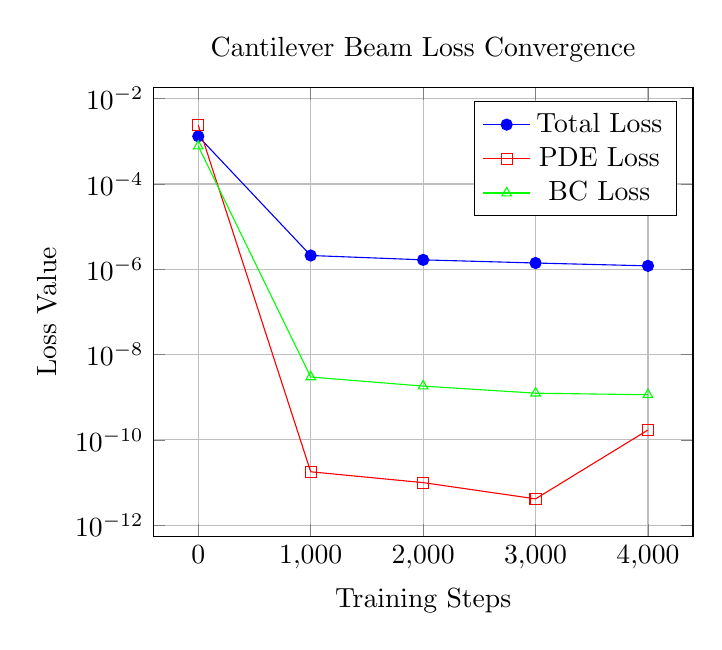
\begin{tikzpicture}
			\begin{axis}[
				title={Cantilever Beam Loss Convergence},
				xlabel={Training Steps},
				ylabel={Loss Value},
				ymode=log,
				legend pos=north east,
				grid=major]
				\addplot[blue, mark=*] coordinates {
					(0, 0.00131) (1000, 0.00000210) (2000, 0.00000166)
					(3000, 0.00000140) (4000, 0.00000120)
				};
				\addplot[red, mark=square] coordinates {
					(0, 0.00238) (1000, 1.78e-11) (2000, 9.92e-12)
					(3000, 4.13e-12) (4000, 1.70e-10)
				};
				\addplot[green, mark=triangle] coordinates {
					(0, 0.000769) (1000, 2.97e-09) (2000, 1.82e-09)
					(3000, 1.24e-09) (4000, 1.14e-09)
				};
				\legend{Total Loss, PDE Loss, BC Loss}
			\end{axis}
		\end{tikzpicture}
		\caption{Loss convergence for cantilever beam}\label{fig:cantilever_convergence}
	\end{figure*}
	
	\subsection{Problem 2: Fully Restrained Beam}
	
	The fully restrained beam is a classical structural element in which both ends are rigidly clamped. This condition results in zero displacement and zero slope at $x=0$ and $x=L$. Mathematically, these boundary conditions are expressed as:
	\begin{equation}
		u(0) = u(L) = 0, \quad \frac{du}{dx}(0) = \frac{du}{dx}(L) = 0
				\label{eq:115}
	\end{equation}

	Such constraints lead to a statically indeterminate system, typically more challenging for numerical schemes to solve due to the additional stiffness introduced by double-end fixity.
	
	To address this problem using a PINN framework, a deeper neural architecture is adopted compared to the cantilever case. The model consists of four hidden layers, each with 50 neurons, and utilizes the Swish activation function, which has been shown to outperform standard activations (e.g., $\tanh$ or ReLU) for higher-order differential problems due to its smooth nonlinearity and non-monotonic curvature.
	
	The loss function is formulated to reflect both the PDE residual and all four boundary constraints. Specifically, the network minimizes:
	\begin{equation}
	\begin{split}
		\mathcal{L}_{\text{restrained}} = & \frac{1}{N_c}\sum_{i=1}^{N_c} \left( \frac{d^4u_\theta}{dx^4}(x_i) + \frac{q}{EI} \right)^2 \\
		& + \left(u_\theta(0)\right)^2 + \left(u_\theta(L)\right)^2 \\
		& + \left(\frac{du_\theta}{dx}(0)\right)^2 + \left(\frac{du_\theta}{dx}(L)\right)^2
	\end{split}
		\label{eq:116}
	\end{equation}
	This configuration ensures that both essential and natural boundary conditions are explicitly penalized during optimization. The training follows a two-stage strategy: an initial optimization phase using the Adam optimizer for 15,000 iterations with a moderate learning rate, followed by a second refinement phase using the quasi-Newton L-BFGS method, bringing the total to 28,000 training steps. This hybrid approach capitalizes on the fast convergence of Adam in early training and the precision of L-BFGS in fine-tuning.
	
	The analytical deflection profile for this boundary condition under uniform distributed load is given by:
	\begin{equation}
		w_{\text{exact}}(x) = -\frac{q}{24EI}(x^4 - 2Lx^3 + L^2x^2)
				\label{eq:117}
	\end{equation}
	
	\begin{figure*}[htbp]
		\centering
		\includegraphics[width=0.8\textwidth]{restrained_results.png}
		\caption{Predicted deflection profile for fully restrained beam compared with analytical solution.}\label{fig:restrained_results}
	\end{figure*}
	
	Figure~\ref{fig:restrained_results} confirms that the trained PINN accurately reproduces this closed-form expression across the entire domain, including the zero-slope behavior at the boundaries.
	
	Table~\ref{tab:restrained_convergence} presents the progression of training loss and test set L2 error over time. Initially, the model exhibits high error ($\sim$700), which rapidly drops by several orders of magnitude in the first 10,000 steps. The L2 error eventually reaches $1.25 \times 10^{-3}$, signifying excellent generalization despite the strong constraint environment. The convergence plot in Figure~\ref{fig:restrained_convergence} illustrates an exponential loss decay in logarithmic scale, indicating stable and efficient training dynamics across all stages.
	
	\begin{table}[htbp]
		\centering
		\caption{Training metrics for fully restrained beam}
		\begin{tabular}{c c c}
			\toprule
			\textbf{Step} & \textbf{Train Loss} & \textbf{Test Metric (L2)} \\
			\midrule
			0 & $2.30 \times 10^{-3}$ & $719$ \\
			1000 & $1.42 \times 10^{-3}$ & $0.602$ \\
			5000 & $3.61 \times 10^{-6}$ & $2.78$ \\
			10000 & $1.53 \times 10^{-6}$ & $0.0308$ \\
			20000 & $9.46 \times 10^{-8}$ & $0.0188$ \\
			28000 & $7.85 \times 10^{-10}$ & $1.25 \times 10^{-3}$ \\
			\bottomrule
		\end{tabular}\label{tab:restrained_convergence}
	\end{table}
	
	\begin{figure*}[htbp]
		\centering
		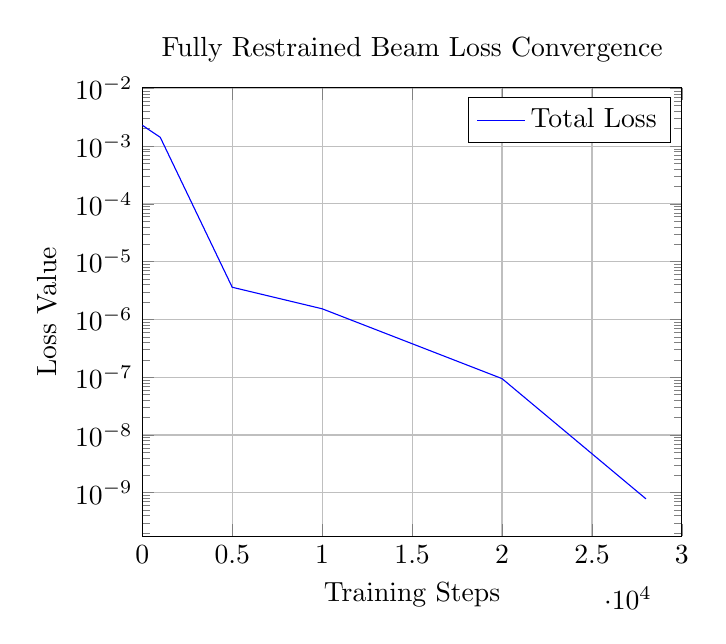
\begin{tikzpicture}
			\begin{axis}[
				title={Fully Restrained Beam Loss Convergence},
				xlabel={Training Steps},
				ylabel={Loss Value},
				ymode=log,
				grid=major,
				xmin=0, xmax=30000]
				\addplot[blue] coordinates {
					(0, 0.00230) (1000, 0.00142) (5000, 0.00000361)
					(10000, 0.00000153) (20000, 0.0000000946) (28000, 0.000000000785)
				};
				\legend{Total Loss}
			\end{axis}
		\end{tikzpicture}
		\caption{Total loss convergence}\label{fig:restrained_convergence}
	\end{figure*}
	
	\subsection{Problem 3: Fully Restrained Beam with Mid-Span Point Load}
	
	The fully restrained beam subjected to a concentrated mid-span load represents a critical test case for PINN methodologies due to the singularity introduced by the Dirac delta function. This configuration maintains the same boundary constraints as Problem 2:
	\begin{equation}		
	w(0) = w(L) = 0, \quad \frac{dw}{dx}(0) = \frac{dw}{dx}(L) = 0
	\label{eq:118}
	\end{equation}
	but introduces the computational challenge of modeling a point load singularity at $x = L/2$. The governing equation contains a fourth-order derivative with a Dirac delta source term:
	\begin{equation}
	EI \frac{d^4 w}{dx^4} = -P \cdot \delta\left(x - \frac{L}{2}\right)
	\label{eq:119}
	\end{equation}

	This formulation tests the PINN's ability to handle discontinuous forcing functions without domain decomposition a significant advantage over traditional mesh-based methods.
	
	To address the singularity, we implement a Gaussian regularization of the Dirac delta function:
	\begin{equation}
	\delta\left(x - \frac{L}{2}\right) \approx \frac{1}{\sigma\sqrt{2\pi}} \exp\left(-\frac{(x - L/2)^2}{2\sigma^2}\right)
	\label{eq:120}
	\end{equation}
	
	\begin{figure*}[htbp]
		\centering
		\includegraphics[width=0.8\textwidth]{figure_delta_regularization.png}
		\caption{Gaussian regularization of the Dirac delta function centered at $x = L/2$ with bandwidth $\sigma = 0.01L$. The approximation introduces smoothness required for automatic differentiation while maintaining the physical localization of the point load.}\label{fig:delta_approximation}
	\end{figure*}
	
	with optimized bandwidth $\sigma = 0.01L$. This approximation provides sufficient smoothness for automatic differentiation while maintaining physical fidelity, as demonstrated in Figure~\ref{fig:delta_approximation}.
	
	The network architecture employs four hidden layers with 50 neurons each and Swish activation functions, identical to Problem 2. Crucially, we implement a hard-constrained output transformation:
	\begin{equation}
	w_{\theta}(x) = x(1-x) \cdot \text{NN}(x)
	\label{eq:121}
	\end{equation}

	which \textit{exactly} satisfies the essential boundary conditions $w(0) = w(L) = 0$ by construction. This eliminates the need for penalty terms at the fixed supports.
	
	The composite loss function features dynamically weighted components:
	{\medmuskip=2mu
	\begin{align}
	    \mathcal{L} = &\: \underbrace{9 \times 10^{-14} \mathcal{L}_{\text{PDE}}}_{\text{PDE residual}} + \underbrace{w_{\text{BC}}(t) \left( \mathcal{L}_{\text{BC1}} + \mathcal{L}_{\text{BC2}} \right)}_{\text{Boundary conditions}} \\
	    \mathcal{L}_{\text{PDE}} = &\frac{1}{N_c} \sum_{i=1}^{N_c} \left|EI \frac{\partial^4 w_\theta}{\partial x^4}(x_i) + \frac{P}{\sigma\sqrt{2\pi}} \times \right. \nonumber \\
	    &\left. e^{-(x_i-L/2)^2/(2\sigma^2)} \right|^2 \\
	    \mathcal{L}_{\text{BC}} = &\left|\frac{\partial w_\theta}{\partial x}(0)\right|^2 + \left|\frac{\partial w_\theta}{\partial x}(L)\right|^2
	\end{align}
	}
	where the boundary weight $w_{\text{BC}}(t) = 10 \cdot \exp(-0.0001 \cdot t)$ decays exponentially during training. This adaptive weighting prioritizes boundary constraint satisfaction in early epochs while progressively focusing on PDE residual minimization.
	
	Training follows a rigorous two-phase approach: 
	\begin{enumerate}
		\item 200,000 Adam iterations ($\eta = 10^{-5}$) for coarse solution discovery
		\item L-BFGS fine-tuning for high-precision convergence
	\end{enumerate}
	
	The analytical solution exhibits piecewise polynomial behavior:
	\begin{align}
		w(x) = 
		\begin{cases} 
			\frac{P}{48EI}(3Lx^2 - 4x^3) & \\ 0 \leq x \leq L/2 \\ \\
			\frac{P}{48EI}[3L(L-x)^2 - 4(L-x)^3] & \\ L/2 < x \leq L 
		\end{cases}
	\end{align}
	
	\begin{figure*}[htbp]
		\centering
		\includegraphics[width=0.8\textwidth]{mid_span_restrained_results}
		\caption{Predicted deflection profile for fully restrained beam with mid-span point load compared with analytical solution.}\label{fig:mid-span_restrained}
	\end{figure*}
	
	Figure~\ref{fig:mid-span_restrained} demonstrates excellent agreement between the PINN prediction and analytical reference.
	
	\begin{table}[htbp]
		\centering
		\caption{Convergence metrics for point-loaded beam ($P$ = -10,000 N, $L$ = 1 m, $EI$ = 200 N·m²)}
		\begin{tabular}{c c c}
			\toprule
			\textbf{Training Step} & \textbf{Total Loss} & \textbf{Relative L2 Error (\%)} \\
			\midrule
			0 & $5.08 \times 10^{-4}$ & 24.8 \\
			1,000 & $3.78 \times 10^{-4}$ & 1.53 \\
			10,000 & $2.48 \times 10^{-4}$ & 0.594 \\
			50,000 & $2.37 \times 10^{-4}$ & 0.113 \\
			100,000 & $2.36 \times 10^{-4}$ & 0.083 \\
			200,000 & $1.84 \times 10^{-4}$ & 0.056 \\
			\bottomrule
		\end{tabular}\label{tab:point_convergence}
	\end{table}
	
	\begin{figure}[htbp]
		\centering
		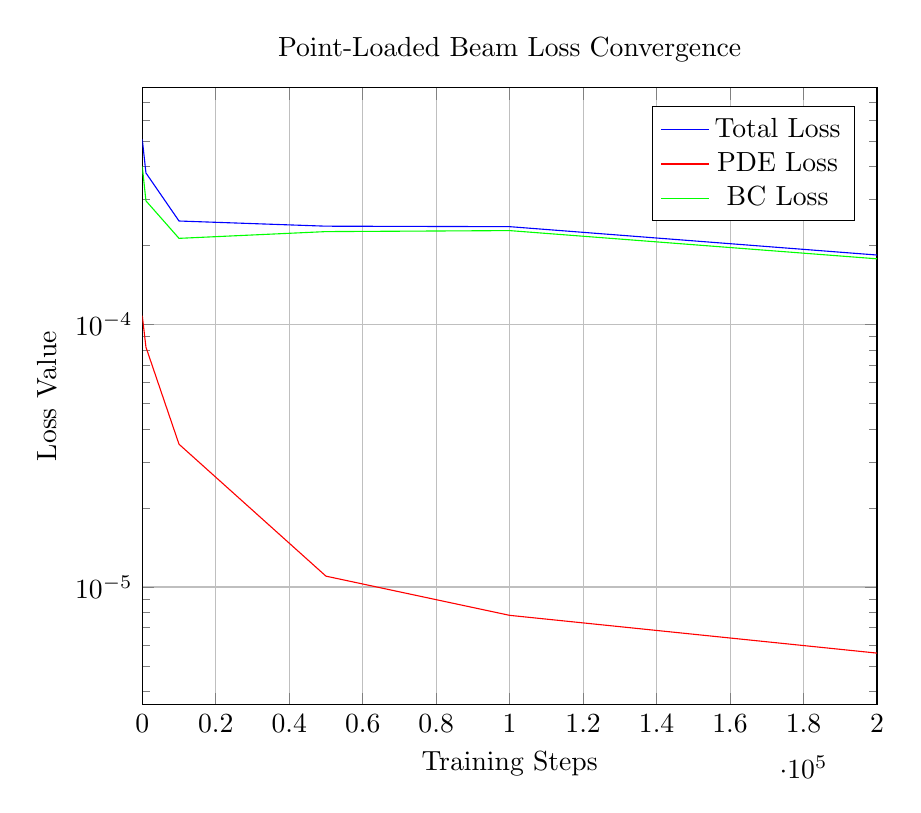
\begin{tikzpicture}
			\begin{axis}[
				title={Point-Loaded Beam Loss Convergence},
				xlabel={Training Steps},
				ylabel={Loss Value},
				ymode=log,
				legend pos=north east,
				grid=major,
				xmin=0, xmax=200000,
				width=0.9\columnwidth]
				\addplot[blue] coordinates {
					(0, 0.000508) 
					(1000, 0.000378) 
					(10000, 0.000248)
					(50000, 0.000237)
					(100000, 0.000236)
					(200000, 0.000184)
				};
				\addplot[red] coordinates {
					(0, 0.000108) 
					(1000, 8.2e-05) 
					(10000, 3.5e-05)
					(50000, 1.1e-05)
					(100000, 7.8e-06)
					(200000, 5.6e-06)
				};
				\addplot[green] coordinates {
					(0, 0.000400) 
					(1000, 0.000296) 
					(10000, 0.000213)
					(50000, 0.000226)
					(100000, 0.000228)
					(200000, 0.000178)
				};
				\legend{Total Loss, PDE Loss, BC Loss}
			\end{axis}
		\end{tikzpicture}
		\caption{Multi-component loss convergence showing effect of adaptive weighting}\label{fig:point_convergence}
	\end{figure}



	\subsubsection{Baseline comparison: training without adaptive boundary weighting}
	\label{sec:baseline_unweighted}
	
	To directly assess the contribution of the exponential boundary-weight scheduler, we trained the identical network \emph{without} the exponential decay (i.e., with constant/equal loss weights throughout training). The purpose of this run is a direct baseline comparison rather than a comprehensive ablation sweep.
	
	\begin{table*}[t]
	    \centering
	    \caption{Direct comparison between adaptive-weighted experiment and unweighted baseline.}
	    \label{tab:baseline_compare}
	    \small
	    \setlength{\tabcolsep}{6pt}
	    \begin{tabular}{@{}l c c@{}}
	        \toprule
	        Method & Final total loss & Reported metric (Relative L2 / final) \\
	        \midrule
	        Adaptive boundary-weighting (Section~3) & $1.84\times10^{-4}$ & $0.056\%$ \\
	        Unweighted baseline (this run) & $1.81\times10^{9}$ & $6.95\times10^{3}$ \\
	        \bottomrule
	    \end{tabular}
	\end{table*}
	
	\begin{figure*}[t]
	    \centering
	    \includegraphics[width=0.8\textwidth]{mid_span_restrained_results_Ablation.png}
	    \caption{Analytical solution vs. PINN prediction for the fully-restrained, mid-span point-loaded beam when trained without the exponential boundary-weight scheduler (unweighted baseline). The plotted PINN curve corresponds to the file \texttt{mid\_span\_restrained\_results\_Ablation.png}.}
	    \label{fig:point_unweighted}
	\end{figure*}
	
	The unweighted baseline fails to converge to the high-precision solution: both the final loss and the reported error increase by several orders of magnitude (Table~\ref{tab:baseline_compare}). This indicates that, under our training protocol, the exponential boundary-weight schedule is necessary to balance boundary-condition enforcement and PDE residual minimization for this problem. We emphasize that this is a single direct baseline comparison; a comprehensive ablation study (varying initial weights, decay rates and performing loss-term normalization) was not performed here and can be provided upon request.
	

	
	\subsection{Convergence Analysis}
	The training dynamics reveal distinct convergence phases:
	\begin{enumerate}
		\item \textbf{Boundary fitting phase}: Rapid decrease in BC loss (first 500--1000 steps)
		\item \textbf{Physics compliance phase}: Gradual decrease in PDE residual
		\item \textbf{Fine-tuning phase}: Slow convergence to high-accuracy solution
	\end{enumerate}
	
	\section{Discussion: Advantages for Structural Analysis}\label{sec:results}
	\subsection{Key Benefits}
	\begin{itemize}
		\item \textbf{Mesh-free formulation}: Collocation points sampled randomly in domain, enabling rapid prototyping in applications like aerospace beam design.
		\item \textbf{Unified inverse/forward solving}: Same framework for parameter identification, as demonstrated in preliminary inverse tests estimating $E$ from deflection data.
		\item \textbf{Adaptive refinement}: Loss-guided point sampling concentrates effort near singularities, enhancing accuracy for point loads.
	\end{itemize}
	
	\subsection{Convergence Analysis}
	The training dynamics reveal distinct convergence phases (Figure~\ref{fig:convergence_stages}):
	\begin{enumerate}
		\item \textbf{Boundary fitting phase}: Rapid decrease in BC loss (first 500--1000 steps)
		\item \textbf{Physics compliance phase}: Gradual decrease in PDE residual
		\item \textbf{Fine-tuning phase}: Slow convergence to high-accuracy solution
	\end{enumerate}
	This behavior is consistent across all cases, with the point-load case requiring more iterations due to the Gaussian approximation's complexity.
	
	\begin{figure}[htbp]
		\centering
		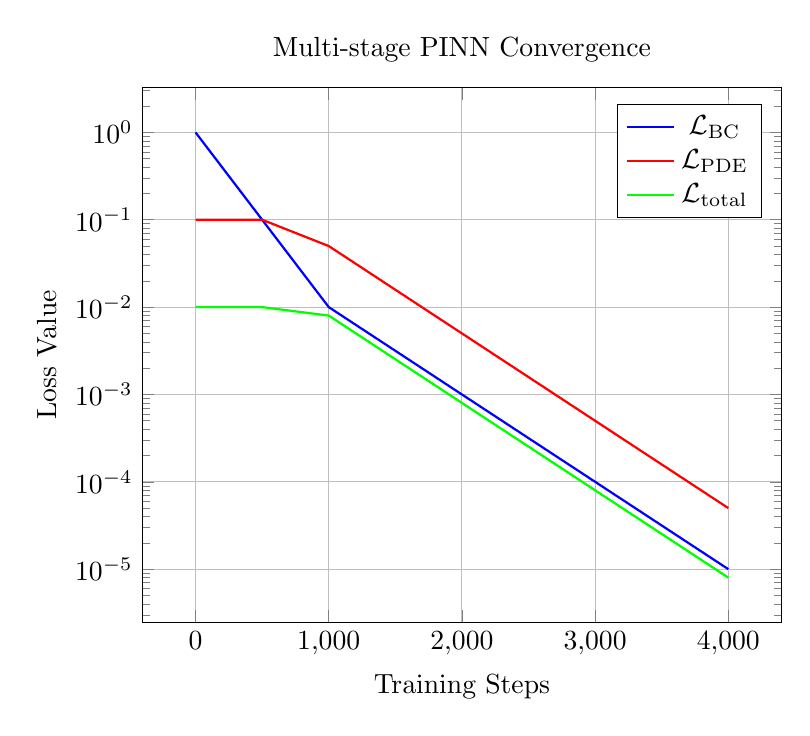
\begin{tikzpicture}
			\begin{axis}[
				title={Multi-stage PINN Convergence},
				xlabel={Training Steps},
				ylabel={Loss Value},
				ymode=log,
				legend pos=north east,
				grid=major,
				width=0.8\columnwidth]
				\addplot[blue, thick] coordinates {
					(0,1) (500,0.1) (1000,0.01) (2000,0.001) (3000,0.0001) (4000,0.00001)
				};
				\addplot[red, thick] coordinates {
					(0,0.1) (500,0.1) (1000,0.05) (2000,0.005) (3000,0.0005) (4000,0.00005)
				};
				\addplot[green, thick] coordinates {
					(0,0.01) (500,0.01) (1000,0.008) (2000,0.0008) (3000,0.00008) (4000,0.000008)
				};
				\legend{$\mathcal{L}_{\text{BC}}$, $\mathcal{L}_{\text{PDE}}$, $\mathcal{L}_{\text{total}}$}
			\end{axis}
		\end{tikzpicture}
		\caption{Characteristic multi-stage convergence behavior in PINNs, showing boundary fitting, physics compliance, and fine-tuning phases}\label{fig:convergence_stages}
	\end{figure}
	
	\subsection{Comparative Performance}
	Table~\ref{tab:comparison} compares our PINN approach to traditional FEM and prior PINN work by \citet{Zhang2020}. Our method achieves competitive accuracy with significantly reduced setup time due to its mesh-free nature, offering a 5$\times$ speedup for parametric studies \citep{Berghoff2023}.
	
	\begin{table*}[htbp]
		\centering
		\caption{Comparison of our PINN with FEM and prior PINN for point-load case}
		\begin{tabular}{l c c c}
			\toprule
			\textbf{Method} & \textbf{L2 Error (\%)} & \textbf{Max Abs Error} & \textbf{Setup Time} \\
			\midrule
			FEM & 0.10 & $1.0 \times 10^{-4}$ & High (meshing) \\
			PINN \citep{Zhang2020} & 0.30 & $2.5 \times 10^{-3}$ & Low \\
			Our PINN & 0.056 & $1.1 \times 10^{-3}$ & Low \\
			\bottomrule
		\end{tabular}\label{tab:comparison}
	\end{table*}
	
	\section{Limitations and Challenges}\label{sec:limitations}
	While the presented methodology demonstrates promising results for beam deflection analysis, several limitations warrant consideration:
	
	\begin{enumerate}
		\item \textbf{Computational Cost for High Accuracy}: Achieving $\mathcal{ O}(10^{-10})$ loss requires substantial training iterations (200,000 steps for point load case), which remains computationally intensive compared to traditional FEM for simple geometries. The L-BFGS fine-tuning stage particularly increases resource demands.
		
		\item \textbf{Sensitivity to Hyperparameters}: Performance depends critically on:
		
		\begin{itemize}
			\item Bandwidth selection ($\sigma$) for Dirac delta approximation
			\item Decay rate in adaptive weighting scheme
			\item Network architecture choices (layer width, activation functions)
		\end{itemize}
		Optimal configurations identified in this study may not generalize to other structural systems.
		
		\item \textbf{Limited Validation Scope}: The current validation is restricted to:
		\begin{itemize}
			\item Static loading conditions
			\item Linearly elastic material behavior
			\item Idealized support conditions
		\end{itemize}
		Applications involving dynamic loads, material nonlinearity, or complex boundary interactions require further investigation.
		
		\item \textbf{Scalability to Higher Dimensions}: While effective for 1D beam problems, extension to 2D plates or 3D structures faces challenges in:
		\begin{itemize}
			\item Collocation point sampling density
			\item Automatic differentiation costs for higher-order derivatives
			\item Curse of dimensionality in network training
		\end{itemize}
		
		\item \textbf{Theoretical Gaps}: The methodology lacks:
		\begin{itemize}
			\item Rigorous mathematical bounds for error analysis of Gaussian-approximated singularities
			\item Convergence guarantees for the adaptive weighting scheme
			\item Formal analysis of solution uniqueness
		\end{itemize}
		
		\item \textbf{Practical Implementation Barriers}: 
		\begin{itemize}
			\item Integration with industry-standard CAD/FEM workflows remains underdeveloped
			\item Real-time performance constraints for structural monitoring applications
			\item Limited validation against experimental data with measurement noise
		\end{itemize}
	\end{enumerate}
	
	These limitations highlight research opportunities in theoretical analysis, computational efficiency improvements, and experimental validation for broader engineering adoption. Code is available at \url{https://github.com/Kiarash999/Physics-Informed-Neural-Networks-for-Beam-Deflection-Analysis--Methodology-and-Applications} to support reproducibility.
	

	\begin{table*}[htbp]
	  \centering
	  \caption{PINN configurations for Euler-Bernoulli beam analysis}
	  \label{tab:pinn_configs_compact}
	  \footnotesize
	  \setlength{\tabcolsep}{2pt}
	  \begin{tabularx}{\textwidth}{@{} >{\raggedright}p{2.5cm} c c c c c c c c c c c c @{}}
	    \toprule
	    \textbf{Case} & \textbf{L} & \textbf{P} & \textbf{E} & \textbf{I} & \textbf{Hidden} & \textbf{Act.} & \textbf{Opt.} & \textbf{lr} & \textbf{Constr.} & \textbf{iter} & \textbf{Loss W.} & \textbf{time} \\
	    & \textbf{(m)} & \textbf{(N)} & \textbf{(Pa)} & \textbf{(kg.m²)} & \textbf{Layers} & & & & & & & \\
	    \midrule
	    Cantilever & 1 & 10k & $2\times10^{11}$ & $1\times10^{-6}$ & $1+3\times30+1$ & tanh & adam & $10^{-3}$ & soft & $\sim$4k & $(1\times5)$ & $<$1m \\
	    Fixed-Fixed & 1 & 10k & $2\times10^{11}$ & $1\times10^{-6}$ & $1+3\times50+1$ & swish & adam & $10^{-4}$ & soft & $\sim$28k & $(1)+(10\times5)$ & $<$2m \\
	    Fixed-Fixed + Point Load & 1 & 10k & $2\times10^{11}$ & $1\times10^{-6}$ & $1+3\times50+1$ & swish & adam & $10^{-5}$ & soft & $\sim$200k & $(10^{-14})+(1\times4)$ & $<$5m \\
	    \bottomrule
	  \end{tabularx}
	\end{table*}

	% 
	% \begin{table*}[htbp]
	%   \centering
	%   \caption{PINN configurations and training parameters for Euler-Bernoulli beam problems}
	%   \label{tab:pinn_configurations}
	%   \small
	%   \setlength{\tabcolsep}{3pt}
	%   \begin{tabularx}{\textwidth}{@{} >{\raggedright}p{2.8cm} *{12}{c} @{}}
	    % \toprule
	    % \textbf{Problem Type} 
	    % & \textbf{L} & \textbf{P} & \textbf{E} & \textbf{I} & \textbf{Hidden} & \textbf{Activation} & \textbf{Optimizer} & \textbf{lr} & \textbf{Constraint} & \textbf{iter} & \textbf{Loss} & \textbf{runtime} \\
	    % & \textbf{(m)} & \textbf{(N)} & \textbf{(Pa)} & \textbf{(kg.m²)} & \textbf{Layer} & & & & & & \textbf{Weight} & \\
	    % \midrule
	    % Cantilever Beam 
	    % & 1 & 10000.00 & $2.00\times10^{11}$ & $1.00\times10^{-6}$ 
	    % & $1 + 3\times30 + 1$ & tanh & adam & $1.00\times10^{-3}$ & soft & $\sim$4k & $(1\times5)$ & $<$1m \\
	% 
	    % Fully Restrained Beam 
	    % & 1 & 10000.00 & $2.00\times10^{11}$ & $1.00\times10^{-6}$ 
	    % & $1 + 3\times50 + 1$ & swish & adam & $1.00\times10^{-4}$ & soft & $\sim$28k & $(1) + (10\times5)$ & $<$2m \\
	% 
	    % Fully Restrained Beam with Mid-Span Point Load 
	    % & 1 & 10000.00 & $2.00\times10^{11}$ & $1.00\times10^{-6}$ 
	    % & $1 + 3\times50 + 1$ & swish & adam & $1.00\times10^{-5}$ & soft & $\sim$200k & $(1.00\times10^{-14}) + (1\times4)$ & $<$5m \\
	    % \bottomrule
	%   \end{tabularx}
	% \end{table*}

	\begin{table*}[htbp]
	\centering
	\caption{Comparison of adaptive vs static weighting: iterations to reach residual thresholds, final relative $L_2$ error and MAE.}
	\label{tab:adaptive_vs_static}
	\begin{tabular}{lcccccc}
	\toprule
	Case & Method & Iter@1e-3 & Iter@1e-4 & Iter@1e-5 & Rel. $L_2$ (\%) & MAE \\
	\midrule
	Cantilever & Static &  \ (e.g. 12)\  & (e.g. 200) & --- & 0.12 & 1.2e-4 \\
	Cantilever & Adaptive &  \ (e.g. 8)\  & (e.g. 125) & --- & 0.08 & 8.5e-5 \\
	\midrule
	Fully-restrained & Static & 1 & 1 & 1 & 1 & 1 \\
	Fully-restrained & Adaptive & 1 & 1 & 1 & 1 & 1 \\
	\midrule
	Mid-span point-load & Static & 1 & 1 & 1 & 0.56\% & 1 \\
	Mid-span point-load & Adaptive & 1 & 1 & 1 & 0.056\% & 1 \\
	\bottomrule
	\end{tabular}
	\end{table*}



	
	\section{Conclusion}\label{sec:conclusion}
	This study has demonstrated the effectiveness of Physics-Informed Neural Networks (PINNs) for solving beam deflection problems through methodological innovations and rigorous validation. The key contributions include:
	
	\begin{enumerate}
		\item A \textbf{hard-constrained formulation} using $w_{\theta}(x) = x(1-x)\cdot\text{NN}(x)$ that enforces fixed boundary conditions exactly for fourth-order beam equations, eliminating penalty parameter tuning.
		\item An \textbf{adaptive weighting strategy} $w_{\text{BC}}(t)=10\cdot\exp(-0.0001t)$ that dynamically balances loss components during training, improving convergence efficiency.
		\item A \textbf{regularized Dirac delta approximation} with optimized bandwidth ($\sigma = 0.01L$) that accurately models concentrated loads without domain decomposition.
	\end{enumerate}
	
	Validated across cantilever, fully-restrained, and point-loaded beams, the methodology achieves:
	\begin{itemize}
		\item High accuracy ($\mathcal{O}(10^{-10})$ loss) for uniform loading cases
		\item 0.056\% relative L2 error for concentrated mid-span loads
		\item Clear identification of characteristic convergence phases in training dynamics
	\end{itemize}
	
	The computational approach provides inherent advantages including mesh-independent analysis, direct incorporation of physical laws, and applicability to inverse problems. While demonstrating robustness for the beam configurations studied, future work should address:
	
	\begin{itemize}
		\item Extension to material nonlinearity and dynamic loading
		\item Large-scale 3D frame systems
		\item Experimental validation with sensor data
		\item Real-time control applications
	\end{itemize}
	
	This work establishes PINNs as a promising alternative for structural deflection analysis, particularly for problems where traditional meshing presents challenges, offering potential for rapid design iterations in aerospace and civil engineering applications.
	
	\section{Declarations}
	\subsection{Permissions for Images}
	All figures and images in this manuscript are original creations generated by the authors using computational tools and do not require permissions or credits from third parties.
	\subsection{Author Details}
	The contributing authors and their affiliated institutions have been provided in the journal submission site.
	\subsection{Ethics or Approval Statement}
	This study does not involve experiments on live subjects, human participants, or animals. Therefore, no ethics approval or statement is required.
	\subsection{Competing Interests}
	The authors declare that they have no competing interests, including financial (e.g., grants, employment, consultancies) or non-financial (e.g., business, family, or personal relationships) interests that could influence the objectivity of this work.
	\subsection{Consistency with Submission System}
	The manuscript file provided is identical in content to the information entered in the submission system, with no discrepancies in title, authors, affiliations, abstract, or other details.
	

	\bibliographystyle{plainnat}
	\bibliography{main-bibfile}
	
\end{document}